The majority of the work completed to date relates to an attempt to familiarise myself with the problem and the literature, and to provide myself with the tools required to achieve the goals set for the thesis. While a large proportion of this is in reading the literature and understanding the state of the art, evidence of which is presented in the literature review, I have produced some tangible outcomes thus far. \\

The first and most significant of these is a simulator for the compass-gait walker (see Figure~\ref{fig:simsample}). This has been implemented in Simulink and invoked with a MATLAB script to allow for easy alteration of the dynamic parameters. At present, this is only capable of simulating the compass-gait walker, but it has been designed in view of being able to be extended (with some effort) to simulating a higher-DOF robotic walker. The simulation and script have also been designed in order that the behaviour of the system is easily analysed. At each footstep, critical information about the robot's state is output, and the simulation is designed to output all relevant data for plotting once the simulation terminates. At present, the impact conditions are overly simple; immediate work in improving the model at impacts is required.\\

\begin{figure}
	\centering
	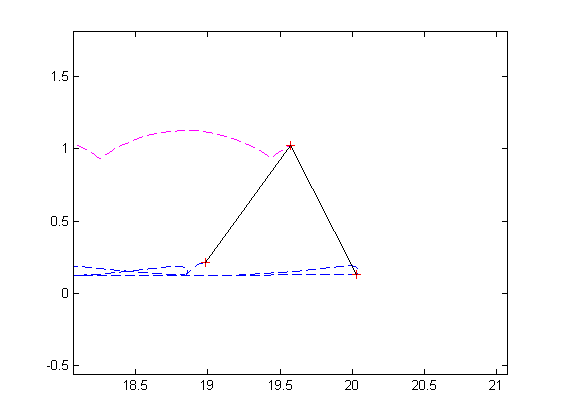
\includegraphics[width=0.8\linewidth]{Images/sim.png}
	\label{fig:simsample}
	\caption{Simulator showing walking compass-gait robot}
\end{figure}

I have implemented a simple high-gain PD controller to regulate a virtual constraint set prior to the start of the simulation. Therefore, at the current time, no path planning has been implemented; the controller enforces a single virtual constraint throughout the simulation. This controller should be altered to better track the desired trajectory by including a component of feedforward control using the model of the hybrid zero dynamics. Also, a motion planner must be designed and implemented as one of the next tasks completed in my thesis work. At present, the simulation detects foot impacts by a condition which is true for horizontal ground. Since this thesis work is intended to allow for path planning over uneven ground, this will need to be updated, along with some means of specifying the terrain. \\

I have created a GUI for designing B{\'e}zier constraints (see Figure~\ref{fig:bezgui}) to assist both in my intuition as to how the control points change the shape of the resulting curve in the compass gait robot's configuration space, and also to allow for possible future work in using the GUI to generate a range of constraints automatically by setting points at the boundaries. The GUI also allows me to assess the performance of the controller by verifying whether the path that the end of the swing leg takes corresponds to the path that is set by the control points. \\

\begin{figure}
	\centering
	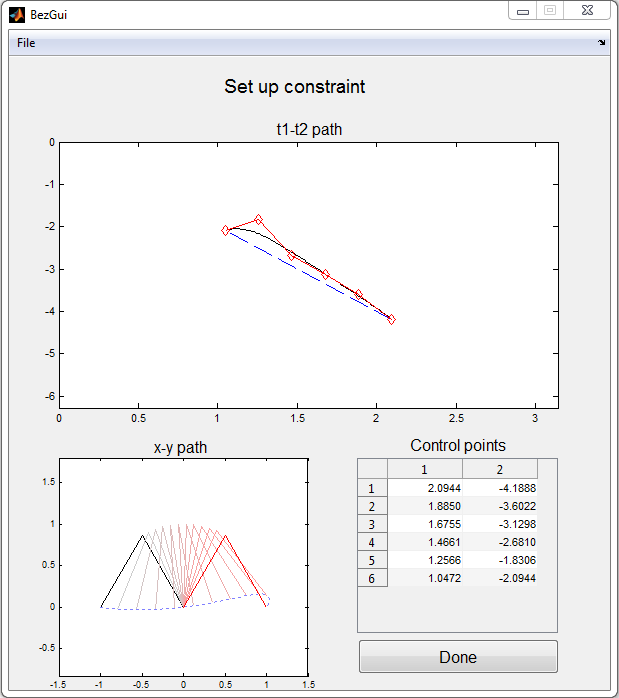
\includegraphics[width=0.8\linewidth]{Images/BezGui.png}
	\label{fig:bezgui}
	\caption{Graphical User Interface for designing B{\'e}zier curve constraints}
\end{figure}

I have begun work on conceptualising an improvement to the energy heuristic used in \cite{manchester13planning}, however this is currently in its early stages; it has not yet been mathematically formalised. At present, the form of the heuristic is as follows: The robot is modelled as a wheeled mass rolling over the terrain. The planner has a maximum and minimum allowable kinetic energy over a receding horizon. The heuristic sets a desired initial kinetic energy such that these limits are upheld. The planner then chooses the footstep in its library of motion primitives which closest matches that kinetic energy and evaluates it for feasibility.